\newcommand{\turnheight}{0.23\columnwidth}
\begin{figure*}
\begin{tabular}{cccc}
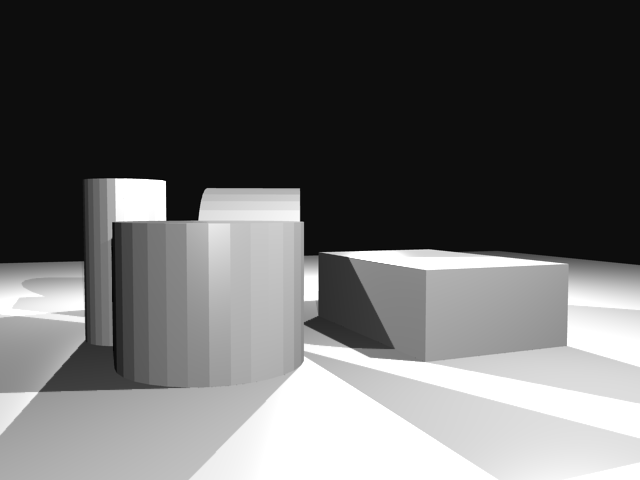
\includegraphics[height=\turnheight]{umk4nke6pzebef2b_SEQ_input.png} &
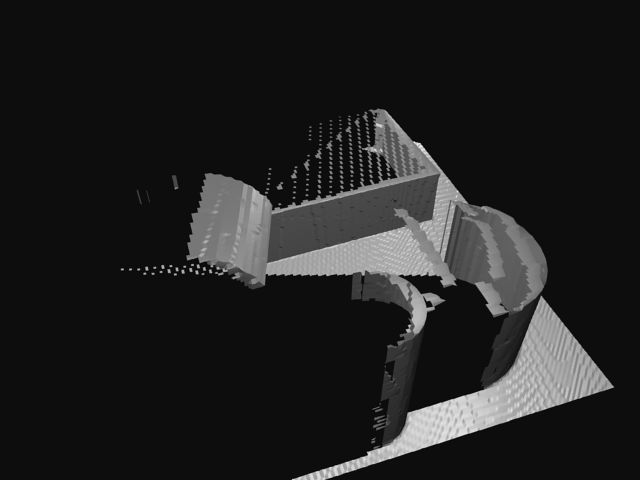
\includegraphics[height=\turnheight]{umk4nke6pzebef2b_SEQ_visible.png} &
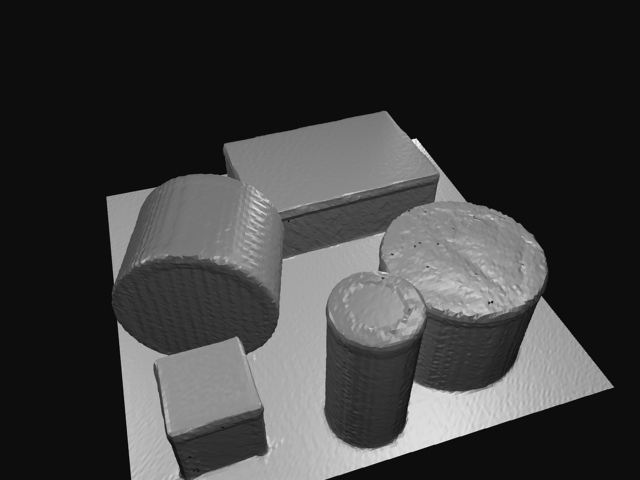
\includegraphics[height=\turnheight]{umk4nke6pzebef2b_SEQ_gt.png} &
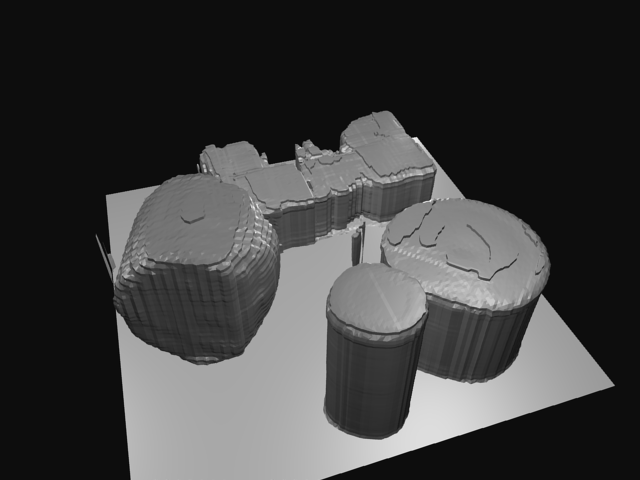
\includegraphics[height=\turnheight]{umk4nke6pzebef2b_SEQ_pred_voxlets.png} \\
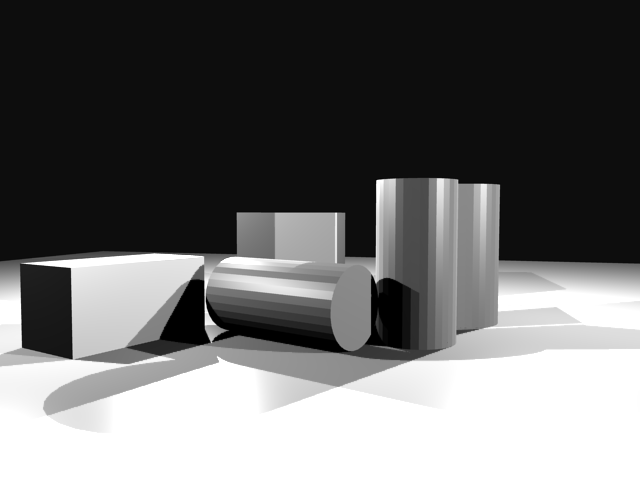
\includegraphics[height=\turnheight]{xf2hcoes8lp9fb1t_SEQ_input.png} &
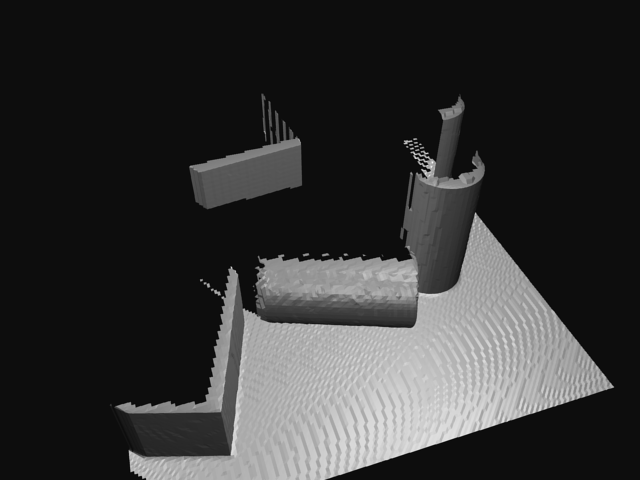
\includegraphics[height=\turnheight]{xf2hcoes8lp9fb1t_SEQ_visible.png} &
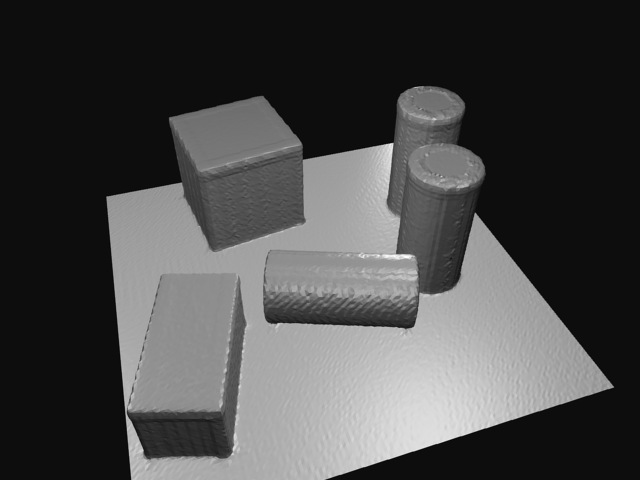
\includegraphics[height=\turnheight]{xf2hcoes8lp9fb1t_SEQ_gt.png} &
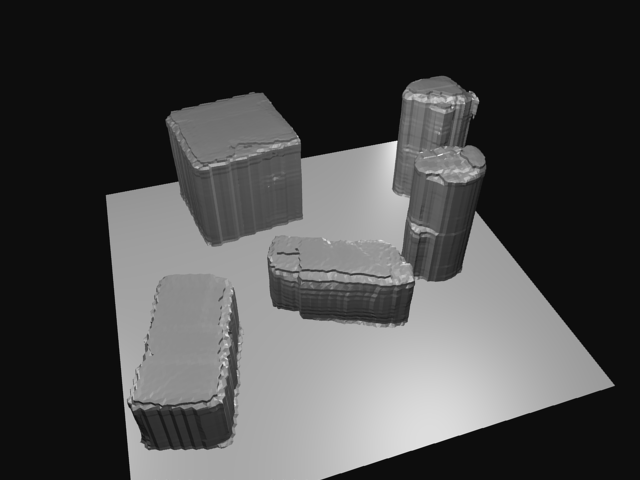
\includegraphics[height=\turnheight]{xf2hcoes8lp9fb1t_SEQ_pred_voxlets.png} \\
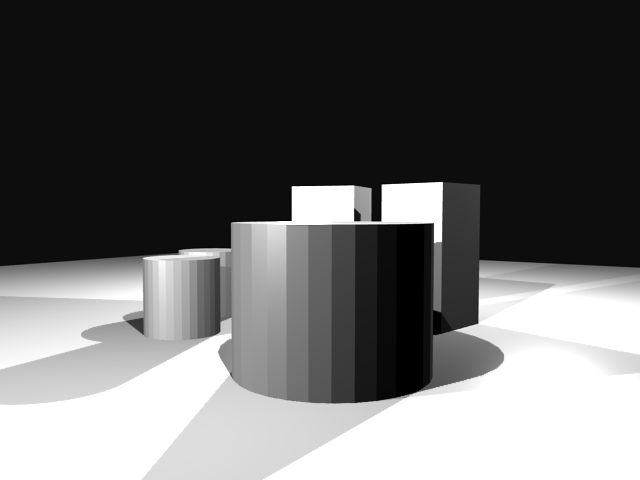
\includegraphics[height=\turnheight]{kmrkmma8u2456lgk_SEQ_input.png} &
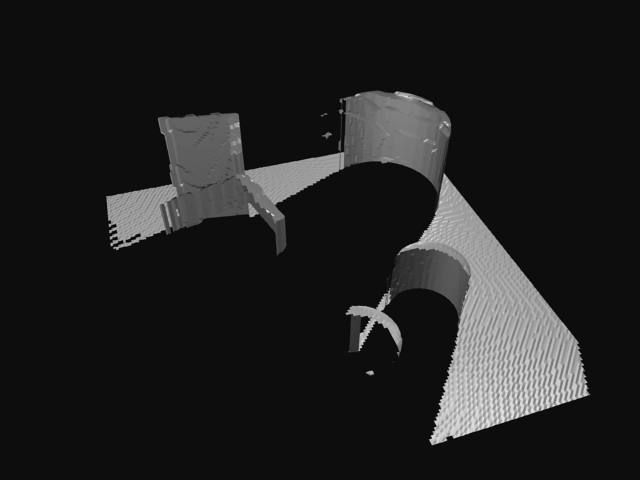
\includegraphics[height=\turnheight]{kmrkmma8u2456lgk_SEQ_visible.png} &
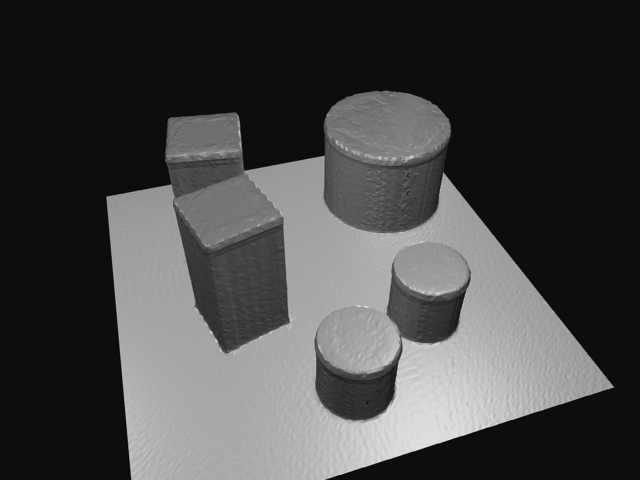
\includegraphics[height=\turnheight]{kmrkmma8u2456lgk_SEQ_gt.png} &
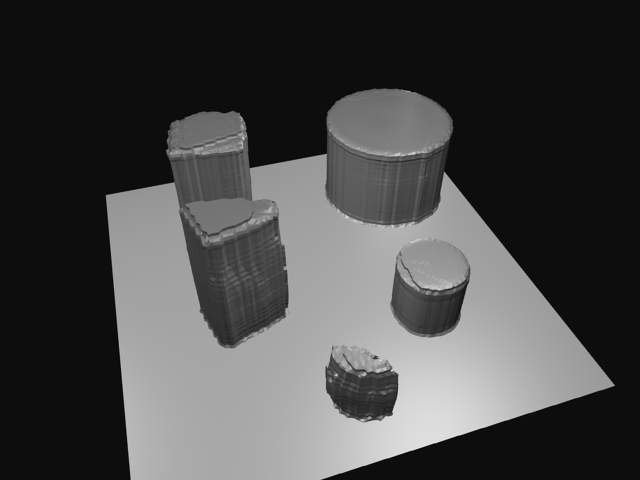
\includegraphics[height=\turnheight]{kmrkmma8u2456lgk_SEQ_pred_voxlets.png} \\
\footnotesize Input view of scene &
\footnotesize Input data in 3D space &
\footnotesize Ground truth occupancy &
\footnotesize Our reconstruction \
\end{tabular}
\end{figure*}
